\documentclass[11pt,a4paper]{article}
\usepackage[a4paper,margin=2.6cm]{geometry}
\usepackage{iftex}
\ifPDFTeX
  \usepackage[T2A]{fontenc}
  \usepackage[utf8]{inputenc}
  \usepackage[russian]{babel}
\else
  \usepackage{fontspec}
  \usepackage{polyglossia}
  \setdefaultlanguage{russian}
  \setotherlanguage{english}
  \defaultfontfeatures{Ligatures=TeX}
  % Font chain: local Times New Roman -> Liberation (Overleaf) -> CMU.
  \IfFontExistsTF{Times New Roman}{%
    \setmainfont{Times New Roman}%
    \setsansfont{Arial}%
    \setmonofont{Courier New}%
    \newfontfamily\cyrillicfont{Times New Roman}%
    \newfontfamily\cyrillicfontsf{Arial}%
    \newfontfamily\cyrillicfonttt{Courier New}%
  }{%
    \IfFontExistsTF{Liberation Serif}{%
      \setmainfont{Liberation Serif}%
      \setsansfont{Liberation Sans}%
      \setmonofont{Liberation Mono}%
      \newfontfamily\cyrillicfont{Liberation Serif}%
      \newfontfamily\cyrillicfontsf{Liberation Sans}%
      \newfontfamily\cyrillicfonttt{Liberation Mono}%
    }{%
      \setmainfont{CMU Serif}%
      \setsansfont{CMU Sans Serif}%
      \setmonofont{CMU Typewriter Text}%
      \newfontfamily\cyrillicfont{CMU Serif}%
      \newfontfamily\cyrillicfontsf{CMU Sans Serif}%
      \newfontfamily\cyrillicfonttt{CMU Typewriter Text}%
    }%
  }
\fi
\usepackage{microtype}
\usepackage{mathtools,amssymb}
\usepackage{graphicx}
\usepackage{booktabs}
\usepackage{float}
\usepackage{caption}
\captionsetup{font=small,labelfont=bf}
\usepackage{enumitem}
\setlist{nosep,leftmargin=1.5em}
\usepackage{csquotes}
\usepackage[backend=biber,style=gost-numeric,sorting=none]{biblatex}
\addbibresource{references_v2.bib}
\usepackage[unicode,hidelinks]{hyperref}
\setlength{\emergencystretch}{2em}

\title{{\normalsize\normalfont\hspace*{-\leftskip}\parbox{\linewidth}{\raggedright УДК~551.513}}\\[1.5em]
Глобальная география сопряжённости иерархических уровней\\
атмосферной циркуляции: атрибуция и планетарная карта}
\author{Сотириади Н.}
\date{2026}

\begin{document}
\maketitle

\begin{abstract}
Пространственная организация атмосферной циркуляции иерархична, и в первой статье серии показано, что сопряжённость соседних масштабных уровней --- мера того, насколько размещение мезомасштабной изменчивости предопределено соседним крупным уровнем, --- является устойчивым региональным инвариантом нижнетропосферной циркуляции. Настоящая работа отвечает на следующий, собственно географический вопрос: что определяет географию этого инварианта. Носителем вместо 39 региональных областей служит мозаичная карта (реанализ ERA5, относительный вихрь на поверхности 850~гПа): 144 ячейки внутри двенадцати равновеликих областей и глобальная сетка из 936 ячеек ($60^\circ$~ю.\,ш.\,--\,$60^\circ$~с.\,ш., два сезона 2023~г.). География сопряжённости оказывается статистически предсказуемой по внешним ковариатам ($R^2=0{,}40$--$0{,}54$ при выбывании целых регионов и секторов долготы, $p=0{,}001$) и эффективно одномерной: одна синоптическая вихревая активность штормовых путей даёт 85\,\% полного качества предсказания. Механизм двухканален: штормовая активность повышает сопряжённость через дисперсионную структуру, отражаемую спектром; конвективный режим понижает её сверх спектра. Карта воспроизводится свободным модельным расчётом без усвоения наблюдений (ранговая корреляция 0,869 при внутреннем пределе метода 0,897) --- она отражает физику атмосферы, а не устройство наблюдательной сети. Потолок надёжности карты составляет $R^2=0{,}914$; заявленные ковариаты объясняют 59\,\% воспроизводимой дисперсии, необъяснённый остаток воспроизводим и не сводится к спектру. Тропический избыток межгодовой изменчивости в двух из трёх очагов глубокой конвекции статистически связан с Междекадным тихоокеанским колебанием; связь с ЭНСО исключена. Прямая проверка подтверждает статичность инварианта: при известной перестройке циркуляции он не опережает стандартные показатели режима; вопрос о медленном многодесятилетнем дрейфе остаётся открытым. Величина, предсказуемая по физическим условиям и картируемая глобально, дополняет аппарат районирования территорий по устройству межуровневых связей.

\smallskip
\noindent\textbf{Ключевые слова:} региональная география, сопряжённость масштабов, атмосферная циркуляция, атрибуция, штормовые пути, конвективный режим, реанализ, свободный модельный расчёт.
\end{abstract}

\section{Введение}
\label{sec:intro}

\subsection{От регионального инварианта к вопросу об атрибуции}

Региональная дифференциация атмосферной циркуляции традиционно описывается климатологией её ведущих организаторов: внетропических штормовых путей \cite{HoskinsValdes1990,Chang2002,Shaw2016} и режимов глубокой конвекции \cite{Houze2004}. В первой статье серии\footnote{Сотириади~Н. Сопряжённость иерархических уровней атмосферной циркуляции как региональный инвариант (первая статья настоящей серии; подана в печать). Протоколы, код и численные результаты обеих работ открыты в едином репозитории: \url{https://github.com/Theclimateguy/Shroedinger}.} к этому описанию добавлена характеристика иного типа: по полю относительного вихря на поверхности 850~гПа построен профиль сопряжённости соседних октавных уровней~$P$ --- мера того, насколько размещение мезомасштабной изменчивости предопределено соседним крупным уровнем, --- и показано, что эта величина удовлетворяет операциональному определению инварианта динамики геосистем \cite{Puzachenko1986,Puzachenko2004,Puzachenko2010} в традиции выделения уровней организации регионального климата \cite{Krenke2019}: она устойчива к смене сезона, года, фазы ЭНСО, источника данных (MERRA-2 \cite{Gelaro2017}) и схемы разбиения территории, содержит воспроизводимую информацию сверх спектра поля и воспроизводится в модельном расчёте, не усваивающем наблюдений. Обоснование самой конструкции, полное операциональное описание процедуры оценивания и каталог проверенных и отвергнутых интерпретаций даны там же и здесь не повторяются.

Настоящая работа ставит следующий, собственно географический вопрос: \emph{что определяет географию инварианта} --- в каких отношениях его карта находится с известными организаторами циркуляции и с экзогенными граничными условиями (орография, конфигурация суши и океана, температура поверхности океана). Ответ проверяет содержательность величины --- атрибутируема ли она физическим условиям --- и открывает её прикладное использование: характеристика, предсказуемая по условиям и картируемая глобально, может служить координатой районирования территорий по устройству межуровневых связей.

Первая попытка атрибуции была предпринята на региональной выборке и закончилась поучительной неудачей: на двенадцати региональных скалярах пять средовых ковариат (модуль широты, сдвиг ветра, климатология конвективной неустойчивости, доля суши, орография) дали при перекрёстной проверке с исключением по одному отрицательную объяснённую дисперсию ($R^2_{\mathrm{LOO}}=-0{,}62$, $p=0{,}65$). Урок методический: двенадцать точек не способны честно вместить ни одно семейство ковариат, и любые содержательные выводы на такой выборке были бы подгонкой. Решение --- смена единицы выборки: переход от региональных скаляров к мозаичной карте, где единицей выступает ячейка мозаики (далее --- тайл) размером в сотни километров, а региональная принадлежность тайлов используется как блокирующий фактор статистики. Число степеней свободы при этом растёт на порядок ($n\approx144$, затем $n\approx936$), а межрегиональные смешения контролируются схемой выбывания целых регионов или секторов долготы.

Задачи работы: (1)~построить тайловую, а затем глобальную карту тонкомасштабного~$P$ с суррогатной поправкой и проверить её согласованность с региональным уровнем первой статьи; (2)~выполнить статистически честную атрибуцию географии карты по заранее заявленным внешним ковариатам, с отрицательным контролем и контрольной мишенью; (3)~проверить природу карты сопоставлением со свободным модельным расчётом; (4)~атрибутировать ранее обнаруженный тропический избыток межгодовой изменчивости по заранее названным климатическим индексам; (5)~проверить прямое следствие статуса инварианта --- гипотезу статичности (разд.~\ref{sec:static}).

Работа сознательно остаётся в рамках эмпирической атрибуции и картирования. Интерпретирующая рамка --- язык квазинеизменных полей ограничений и функционалов инвариантной меры --- вынесена в завершающую, третью статью серии; здесь она затрагивается лишь в объёме одного раздела~\ref{sec:interp}.

\subsection{Гипотеза статичности}

Величина~$P$ заявлена в первой статье как \emph{статичный} инвариант сложившегося циркуляционного режима: характеристика архитектуры уже установившейся организации, а не переменная, несущая собственную динамику. Из этого статуса вытекает прямое и проверяемое следствие: при перестройке режима такая величина не должна опережать перестройку и не должна превосходить по чувствительности стандартные показатели среднего поля. Это следствие --- не дополнительное ограничение, навешиваемое на результат, а необходимое свойство инварианта, подлежащее проверке наравне с остальными; ей посвящён раздел~\ref{sec:static}.

\section{Материалы и методы}
\label{sec:data}

\subsection{Две части единого протокола}

Материал обеих частей --- реанализ ERA5 \cite{Hersbach2020,Soci2024}: составляющие ветра на изобарической поверхности 850~гПа, сетка $0{,}25^\circ$, шаг 6~ч, поле относительного вихря --- идентично первой статье серии. Обе части выполнены по единому протоколу, зафиксированному до вычислений (все критерии, пороги и нуль-модели заданы заранее; отступления фиксировались в журнале протокола).

\emph{Часть~A} --- 144 тайла внутри двенадцати равновеликих областей первой статьи (12 областей $\times$ 12 тайлов): сетка $3\times4$ на область, ячейки $\approx667\times700$~км. Используются только данные, уже имевшиеся на диске программы (окна 2021--2024~гг.).

\emph{Часть~B} --- глобальная сетка из 936 тайлов: широтные полосы по $6^\circ$ ($\approx$667~км), долготные ячейки по 700~км на центральной широте полосы (точное кольцевое покрытие без остатка), пояс $60^\circ$~ю.\,ш.\,--\,$60^\circ$~с.\,ш.; два независимых сезона --- январь--март и июль--сентябрь 2023~г. Из анализа исключены 34 тайла со средней высотой рельефа более 1200~м (поверхность 850~гПа ниже подстилающей); в атрибуции участвуют 902 тайла.

\emph{Целевая величина} --- тонкомасштабный профиль~$P$ с суррогатной поправкой: сопряжённость огибающих в диапазоне полос 50--400~км, вычисленная по внутренней маске тайла и взятая в превышении над медианой 99 фазовых суррогатов, генерируемых отдельно для каждой пары <<тайл--окно>>. Методика идентична первой статье и здесь не пересказывается.

Полосы 50--400~км частично или полностью лежат ниже эффективного разрешения реанализа: правило 4--7 шагов сетки даёт для ERA5 около 125--220~км \cite{Skamarock2004}, прямая спектральная оценка --- 500--600~км в средних широтах и порядка 1000~км в тропиках \cite{Bolgiani2022}. Работа с тонкими полосами тем не менее корректна по трём причинам. Суррогатная поправка сравнивает наблюдаемое поле с полем той же спектральной структуры, прошедшим тот же вычислительный тракт, --- вклад численной диссипации и параметризаций одинаков в измеряемой величине и в вычитаемом фоне. Карта воспроизводится свободным расчётом другой конфигурации модели на общей сетке $0{,}5^\circ$ на 97\,\% достижимого согласия (разд.~\ref{sec:model}) --- тонкополосная структура не является артефактом конкретного тракта усвоения. Наконец, мозаичная карта согласована с региональным уровнем первой статьи ($\rho=0{,}874$), где сигнатура выдерживает контроль, ограниченный разрешёнными ступенями. Остающееся ограничение обсуждается в разд.~\ref{sec:limitations}.

\subsection{Ковариаты и их причинный статус}

Внешние ковариаты разбиты на два яруса, и граница между ними задана протоколом \emph{до} вычислений --- она определяет допустимый язык интерпретации, а не подбирается под результат.

\emph{Ярус~1 --- экзогенные граничные условия} (допустим направленный язык <<формируют>>): средняя высота и стандартное отклонение орографии, доля суши, дисперсия береговой линии, модуль широты, средний градиент температуры поверхности океана.

\emph{Ярус~2 --- совместно складывающиеся характеристики состояния} (только язык совместной организации, без направленности): климатология конвективной доступной потенциальной энергии CAPE за 2021--2024~гг. \cite{RiemannCampe2009} и синоптическая кинетическая энергия вихрей --- дисперсия ветра относительно скользящего 5-суточного среднего, стандартная мера активности штормовых путей, восходящая к классическим полосовым климатологиям синоптической изменчивости \cite{Blackmon1976,HoskinsHodges2019}.

\emph{Отрицательный контроль} --- индекс листовой поверхности (климатология ERA5, сумма компонент низкой и высокой растительности): биологический показатель, механистически неправдоподобный как фактор сопряжённости масштабов 50--400~км на уровне 850~гПа. Ожидаемый исход --- отсутствие прироста предсказания; значимый прирост означал бы скрытое смешение в схеме, а не открытие.

\subsection{Статистическая схема}

\emph{Нуль-модели атрибуции.} В части~A нулевое распределение строится перестановками региональных меток целыми блоками тайлов (999 повторов): тайлы одного региона всегда перемещаются вместе, поэтому внутрирегиональная зависимость сохраняется в нуле. В части~B нуль --- циклический поворот долготной сетки ковариат относительно карты~$P$ на случайный сдвиг не менее $30^\circ$ (999 повторов). Поворот сохраняет полную пространственную автокорреляцию обоих полей и, поскольку модуль широты инвариантен относительно поворота долготы, сохраняет и всю зональную структуру целиком: значимость теста удостоверяет именно \emph{незональную}, долготную часть атрибуции --- привязку карты к фактическому положению штормовых путей и конвективных очагов, а не только к широтному градиенту.

\emph{Проверка предсказания} --- выбывание целыми блоками: по региону (часть~A) либо по одному из шести секторов долготы по $60^\circ$ (часть~B); сообщаемое $R^2$ всегда относится к предсказанию на не участвовавших в подгонке блоках.

\emph{Эффективная размерность} --- прямой пошаговый отбор ковариат с тем же блочным выбыванием; $k_{80}$ --- число ковариат, достаточное для 80\,\% полного качества.

\emph{Потолок надёжности карты} --- внутрисезонное расщепление выборки пополам: сроки каждой пары <<тайл--сезон>> делятся по чётности на две непересекающиеся половины, каждая половина анкорируется на собственных 99 суррогатах, надёжность полной выборки восстанавливается поправкой Спирмена--Брауна \cite{Spearman1910,Brown1910}. Подчеркнём выбор именно внутрисезонной оценки: межсезонная согласованность двух карт ($r=0{,}776$) занижает потолок, поскольку списывает реальное сезонное изменение карты на счёт шума.

\emph{Контрольная (плацебо) мишень} --- наклон пространственного спектра тайла: если бы атрибуция~$P$ лишь повторяла атрибуцию спектра, нагрузки двух мишеней совпадали бы.

\section{Результаты}
\label{sec:results}

\subsection{Часть A: тайлы внутри регионов}
\label{sec:armA}

Итоги части сведены в табл.~\ref{tab:armA}; внутренняя география областей показана на рис.~\ref{fig:tiles}, диаграммы атрибуции --- на рис.~\ref{fig:attrA}.

\begin{table}[t]
\centering
\caption{Часть A: сводка проверок на 144 тайлах внутри 12 равновеликих областей. LOO --- выбывание по региону; блочный нуль --- перестановки на уровне регионов.}
\label{tab:armA}
\small
\begin{tabular}{@{}p{0.44\linewidth}p{0.50\linewidth}@{}}
\toprule
Проверка & Итог\\
\midrule
Согласованность с региональным уровнем первой статьи & $\rho=0{,}874$ (заранее заданный порог 0,7)\\
Атрибуция, выбывание по региону & $R^2=0{,}404$; $p=0{,}001$\\
Определяющие факторы внутри регионов (устраняет межрегиональные смешения) & CAPE: $\rho=-0{,}61$, $p=0{,}002$, знак согласован в 10 из 12 регионов; вихревая энергия: $\rho=+0{,}59$, $p=0{,}002$, в 11 из 12; орография, доля суши, береговая линия --- незначимы на уровне тайла\\
Контрольная мишень: атрибуция наклона спектра & $R^2=0{,}31$, $p=0{,}004$, но с иными нагрузками (орография $+0{,}82$, суша $+0{,}67$, CAPE и вихревая энергия $\approx0$)\\
\bottomrule
\end{tabular}
\end{table}

В части~A участвуют пять из восьми ковариат (стандартное отклонение орографии, доля суши, дисперсия береговой линии, CAPE, вихревая энергия): модуль широты, градиент температуры поверхности океана и средняя орография практически вырождены внутри отдельной области и информативны только на глобальной сетке. Атрибуция состоялась: пять внешних ковариат предсказывают тайловый~$P$ вне региона подгонки ($R^2=0{,}404$ при 95-м перцентиле нуля $-0{,}01$), и два фактора выдерживают самую жёсткую проверку --- корреляцию \emph{внутри} регионов, которую не может породить никакое межрегиональное смешение: конвективный режим (CAPE) понижает сопряжённость, синоптическая вихревая активность повышает её. Контрольная мишень показывает, что это не пересказ спектра: наклон спектра тоже атрибутируем, но совершенно другими ковариатами (орография и доля суши), так что заранее заявленное условие <<спектрального опосредования>> не срабатывает.

Дополнительное, описательное (апостериорное, помеченное так и в протоколе) двухслойное прочтение уточняет механизм. Если перед атрибуцией удалить из тайлового~$P$ часть, линейно предсказуемую по спектральным признакам самого тайла, совместная атрибуция исчезает ($R^2=-0{,}06$), однако отрицательная связь с CAPE выживает внутри регионов (10 из 12, средняя $\rho=-0{,}34$), а связь с вихревой энергией --- нет (8 из 12, $\rho\approx+0{,}03$). Отсюда двухканальная картина: \emph{штормовая активность повышает сопряжённость преимущественно через ту же дисперсионную структуру, которую видит спектр; глубокая конвекция понижает её сверх того, что видит спектр}. Интермиттентная, локально порождаемая завихренность мезомасштабных конвективных систем \cite{Houze2004} расцепляет соседние масштабы; организованные бароклинные возмущения штормовых путей их связывают.

\begin{figure}[t]
\centering
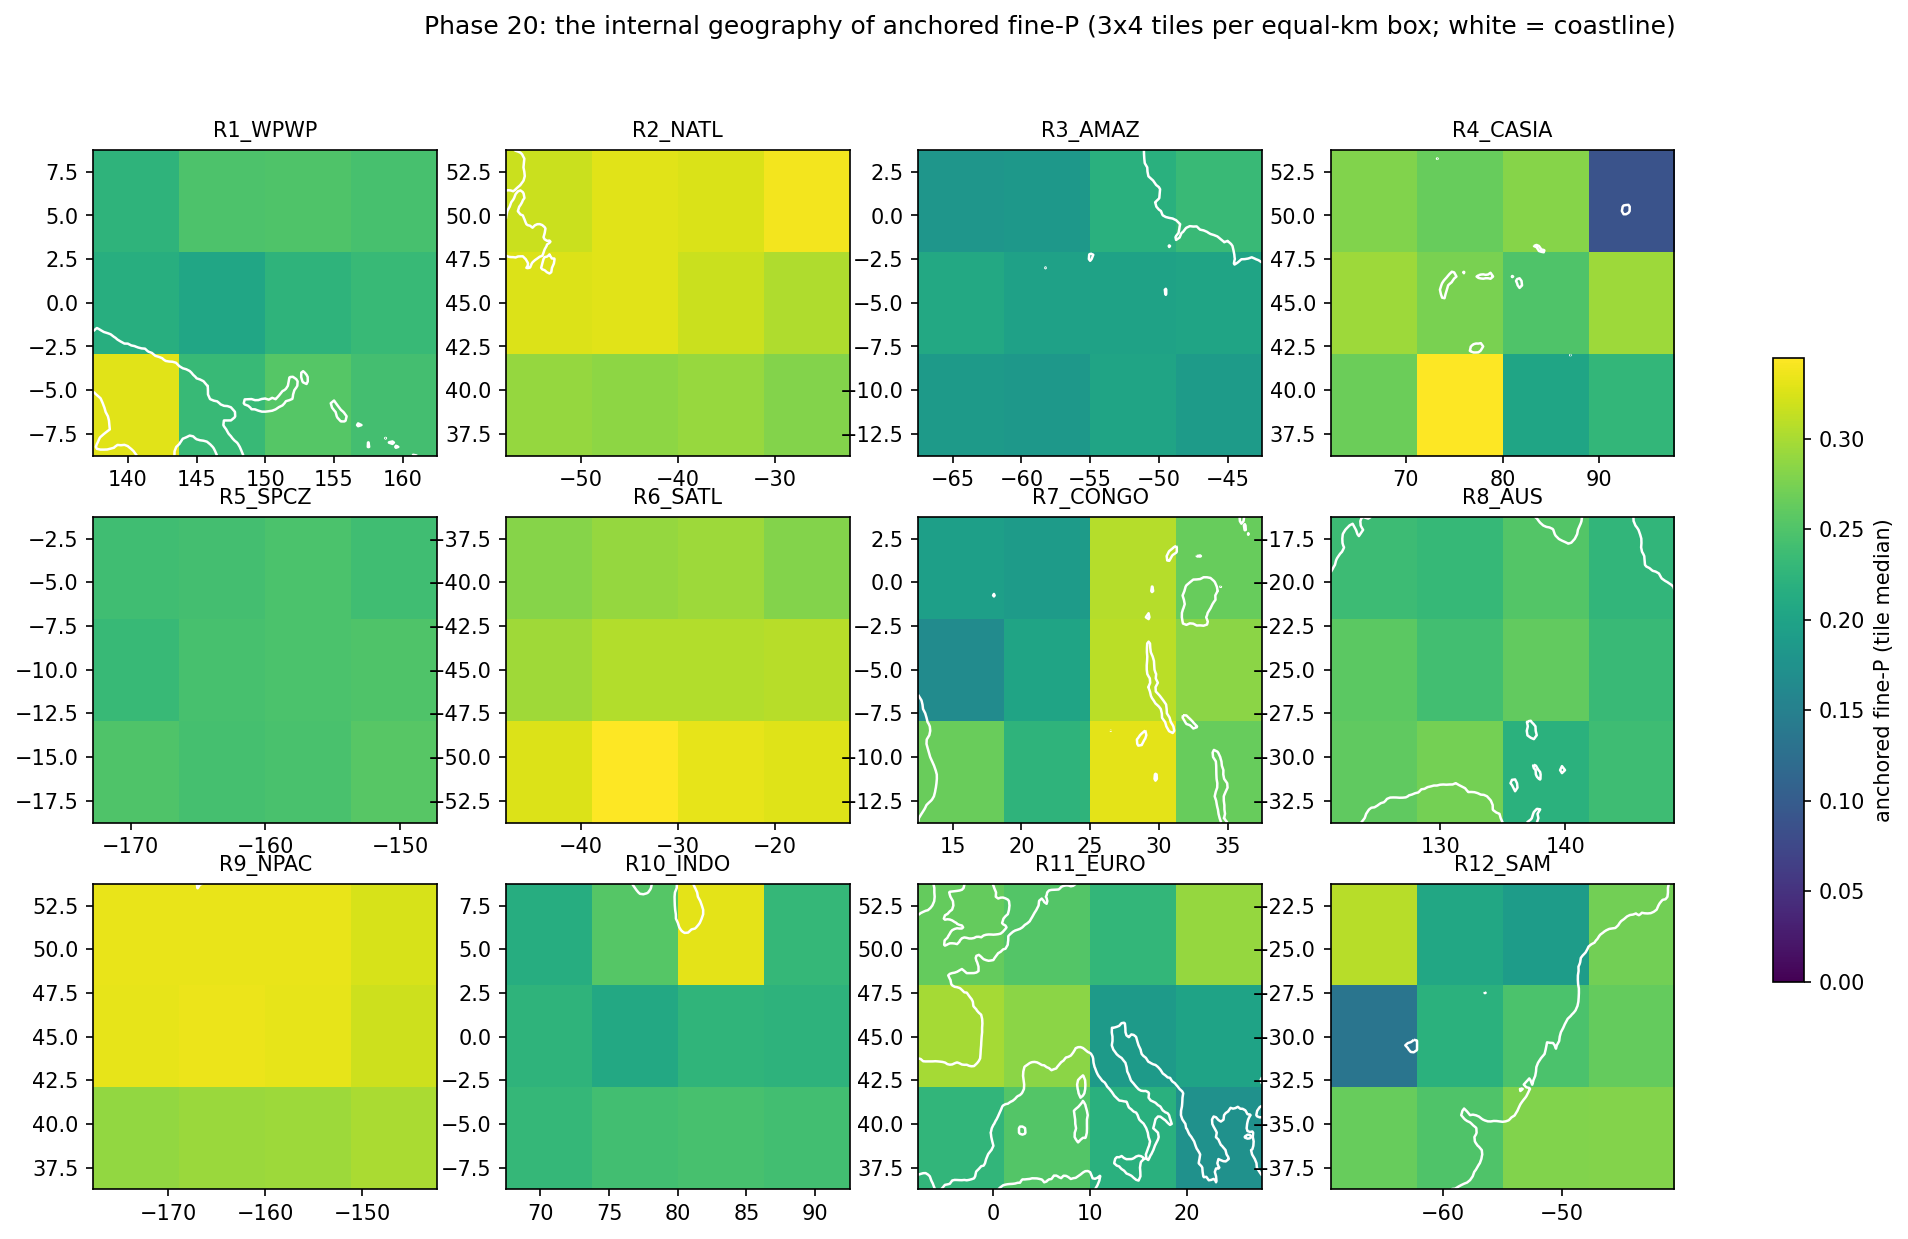
\includegraphics[width=\linewidth]{figures/fig2_tile_maps.png}
\caption{Внутренняя география тонкомасштабного $P$ с суррогатной поправкой (полосы 50--400~км): 12 равновеликих областей $\times$ 12 тайлов, медианы по окнам; белым --- береговая линия. Максимумы --- области штормовых путей (R2, R6, R9), минимумы --- ядра глубокой конвекции (запад Конго, Амазония) и северо-восточный тайл Центральной Азии.}
\label{fig:tiles}
\end{figure}

\begin{figure}[t]
\centering
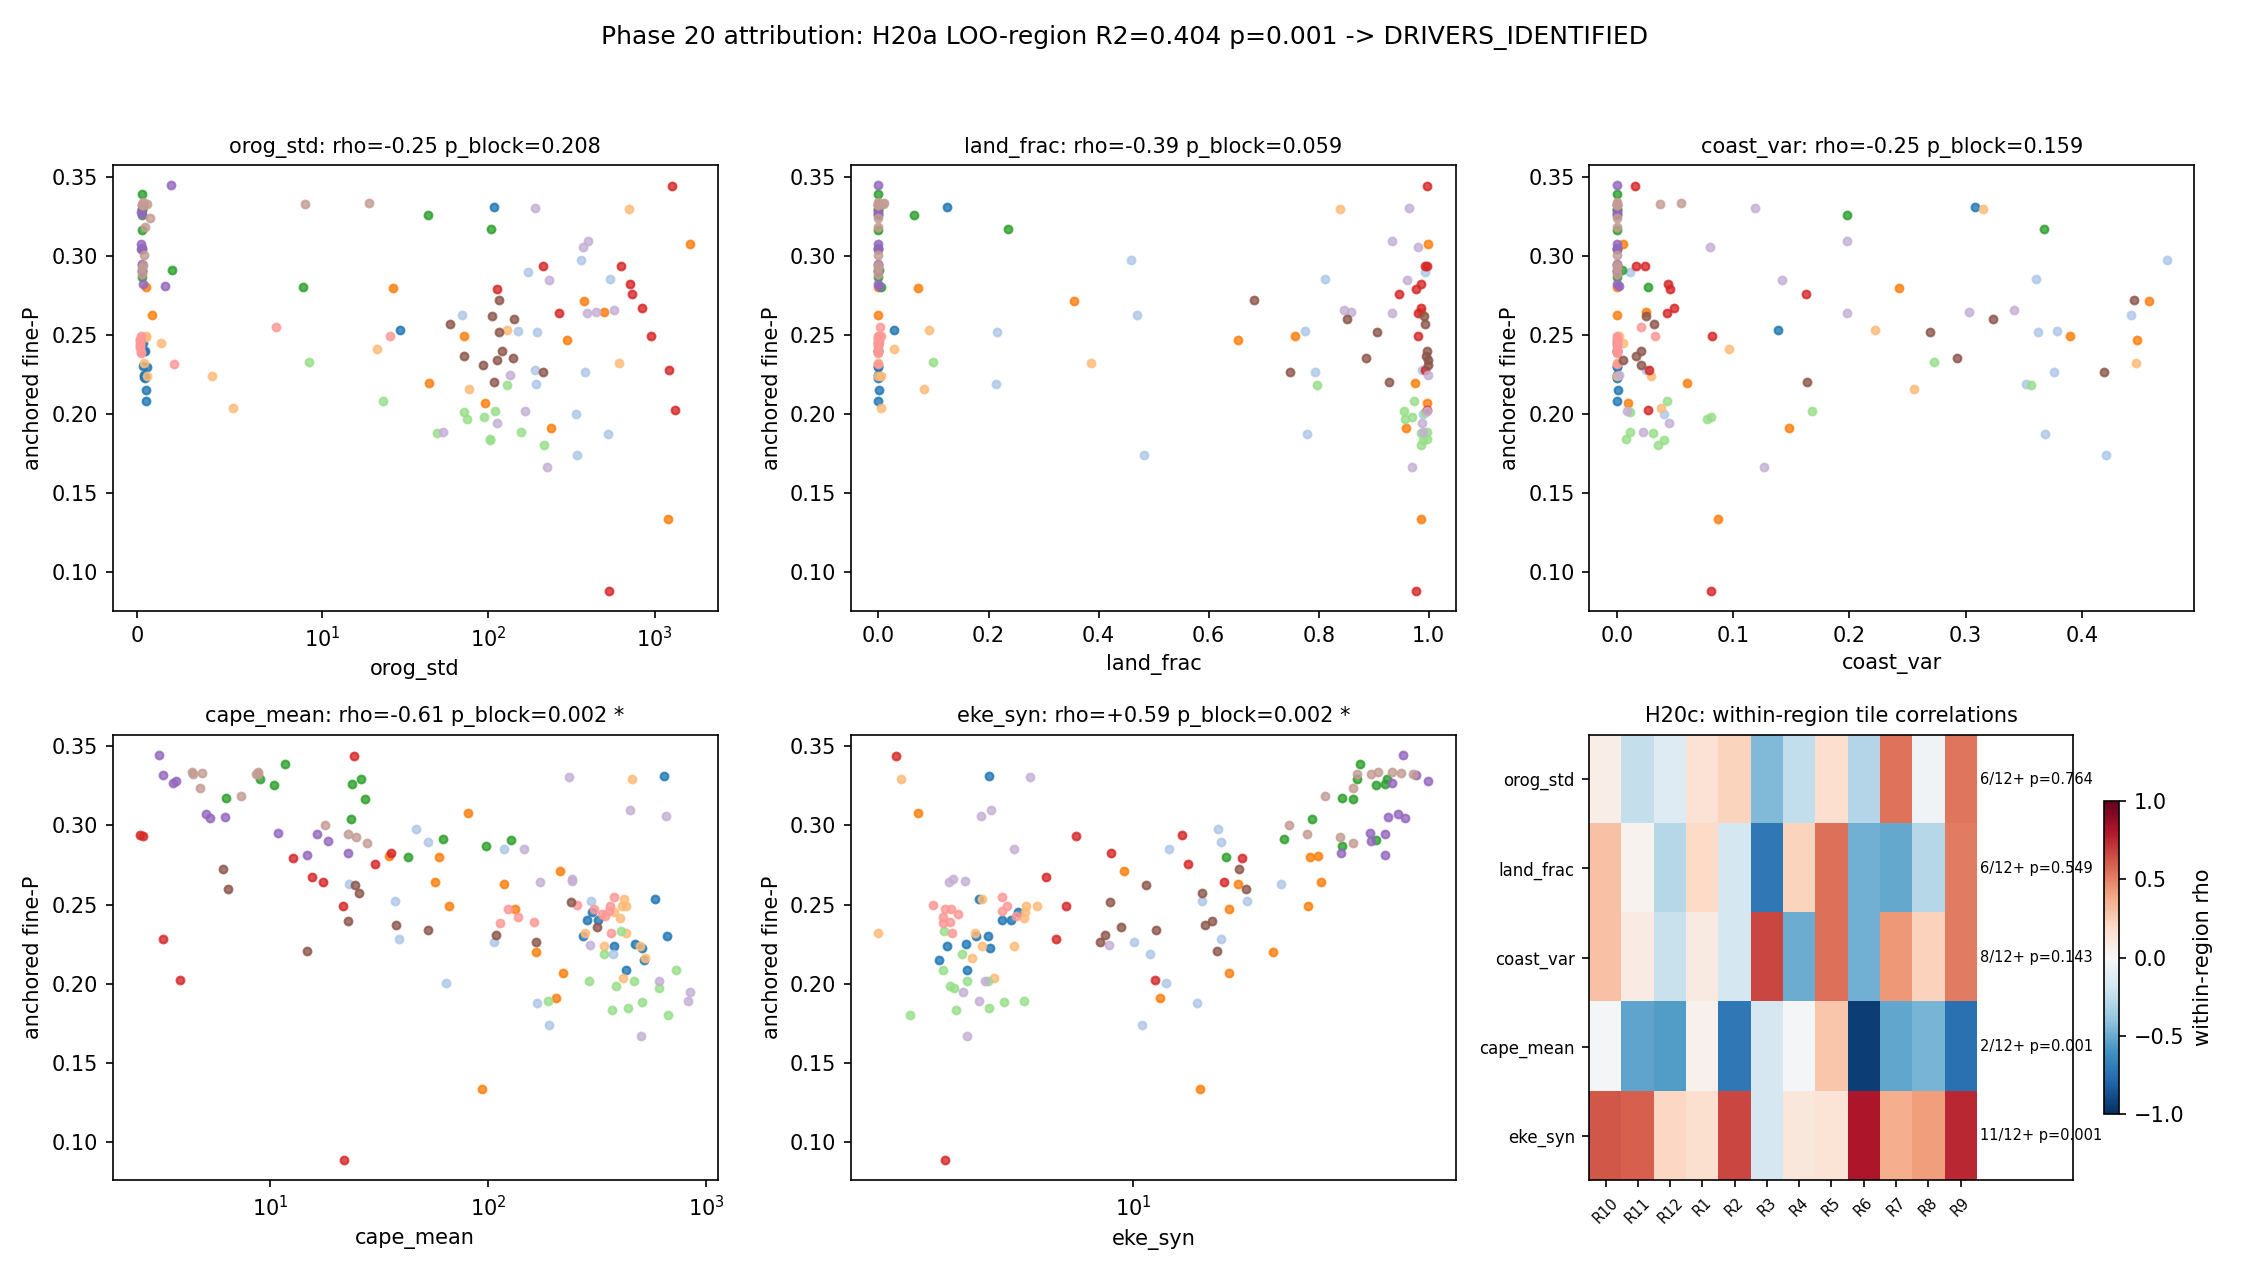
\includegraphics[width=\linewidth]{figures/fig2_attribution.png}
\caption{Часть A, атрибуция тайлового $P$: диаграммы рассеяния по пяти ковариатам с $p$-значениями блочного нуля (цвет --- регион; звёздочкой отмечены значимые связи) и тепловая карта внутрирегиональных корреляций (справа внизу): CAPE отрицательна в 10 из 12 регионов, синоптическая вихревая энергия положительна в 11 из 12.}
\label{fig:attrA}
\end{figure}

\subsection{Часть B: глобальная карта}
\label{sec:armB}

Глобальная карта тонкомасштабного~$P$ с суррогатной поправкой --- центральный результат работы (рис.~\ref{fig:global}); сводка проверок --- в табл.~\ref{tab:armB}, посезонные карты и нагрузки --- на рис.~\ref{fig:seasons}.

\begin{figure}[t]
\centering
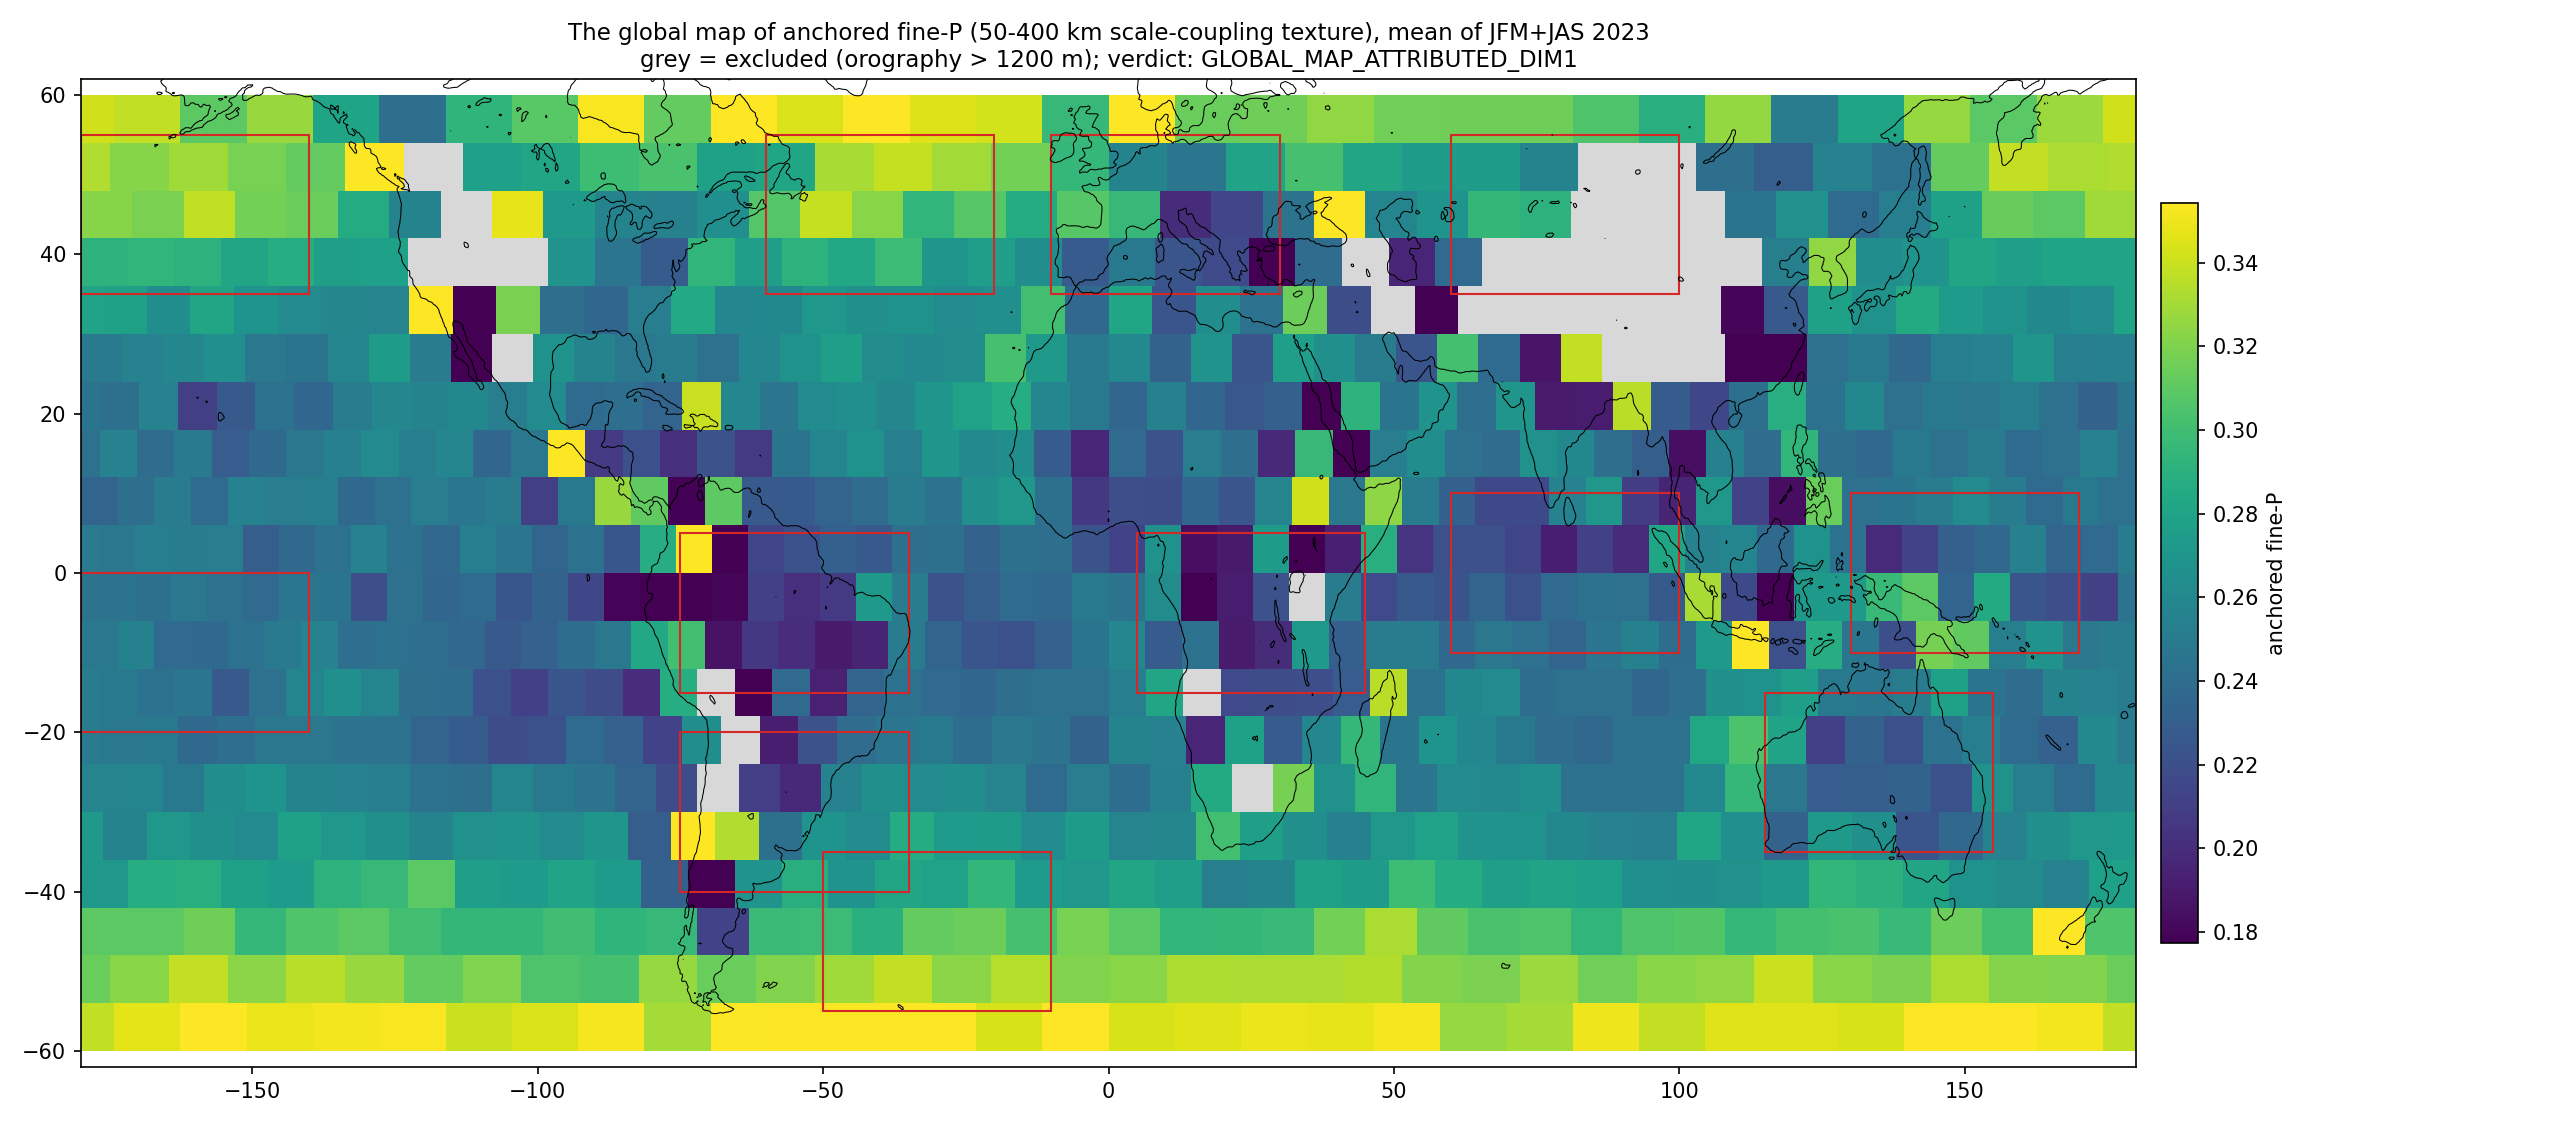
\includegraphics[width=\linewidth]{figures/fig2_global_map.png}
\caption{Глобальная карта тонкомасштабного $P$ с суррогатной поправкой (сопряжённость полос 50--400~км), среднее сезонов январь--март и июль--сентябрь 2023~г., 936 тайлов, $60^\circ$~ю.\,ш.\,--\,$60^\circ$~с.\,ш. Серым --- тайлы, исключённые по орографии (средняя высота более 1200~м); красные рамки --- двенадцать областей программы. Максимумы --- кольцо штормовых путей Южного океана и штормовые пути севера Тихого и Атлантического океанов; минимумы --- Амазония, бассейн Конго, зона муссонной конвекции Морского континента.}
\label{fig:global}
\end{figure}

\begin{table}[t]
\centering
\caption{Часть B: сводка проверок на глобальной сетке (902 тайла после орографического исключения). LOSO --- выбывание по сектору долготы $60^\circ$; нуль --- вращение долготной сетки ковариат (999 повторов).}
\label{tab:armB}
\small
\begin{tabular}{@{}p{0.46\linewidth}p{0.48\linewidth}@{}}
\toprule
Проверка & Итог\\
\midrule
Согласованность с частью A (133 общих тайла) & $\rho=0{,}840$ (заранее заданный порог 0,7)\\
Атрибуция, выбывание по сектору & $R^2=0{,}536$; $p=0{,}001$ (95-й перцентиль нуля 0,455)\\
Разделение по ярусам & ярус 1 (граничные условия): $R^2=0{,}482$ ($p=0{,}002$); прирост от яруса 2: $+0{,}053$\\
Эффективная размерность & одна вихревая энергия: $R^2=0{,}456$, т.\,е. 85\,\% полного качества; $k_{80}=1$\\
Потолок надёжности карты (внутрисезонное расщепление пополам) & $R^2=0{,}914$; атрибуция объясняет 59\,\% воспроизводимой дисперсии\\
Контрольная мишень: наклон спектра & $R^2=0{,}57$, но с иными нагрузками (орография, суша --- вместо вихревой энергии, широты, ТПО, CAPE)\\
Отрицательный контроль (индекс листовой поверхности) & прирост $-0{,}004$; $p=0{,}832$ --- контроль чист\\
Сезонная устойчивость карты & медиана $\lvert$ЯФМ$-$ИАС$\rvert=0{,}016$ (ЯФМ --- январь--март, ИАС --- июль--сентябрь) (90-й перцентиль 0,048)\\
\bottomrule
\end{tabular}
\end{table}

Нагрузки ковариат на поправленный профиль~$P$: вихревая энергия $+0{,}66$; модуль широты $+0{,}66$; градиент температуры поверхности океана $+0{,}55$; CAPE $-0{,}52$; орография и доля суши $\approx0$. У контрольной мишени (наклона спектра) нагрузки противоположного состава: орография $+0{,}74$, доля суши $+0{,}67$, вихревая энергия и CAPE~$\approx0$ (табл.~\ref{tab:loadings}). Двухканальный механизм части~A воспроизводится глобально: сопряжённость уровней и форма спектра управляются \emph{разными} наборами условий, и атрибуция~$P$ не сводится к атрибуции спектра. География максимумов при этом согласуется с классической климатологией и динамикой штормовых путей обоих полушарий \cite{HoskinsValdes1990,Chang2002,Shaw2016}.

\begin{table}[t]
\centering
\caption{Нагрузки ковариат (ранговая корреляция по 902 тайлам) на две мишени: $P$ с суррогатной поправкой и наклон пространственного спектра. Разные наборы ведущих ковариат иллюстрируют двухканальный механизм.}
\label{tab:loadings}
\small
\begin{tabular}{@{}lcc@{}}
\toprule
Ковариата & $P$ с поправкой & Наклон спектра\\
\midrule
Синоптическая вихревая энергия & $+0{,}66$ & $\approx0$\\
Модуль широты & $+0{,}66$ & ---\\
Градиент температуры поверхности океана & $+0{,}55$ & ---\\
Климатология CAPE & $-0{,}52$ & $\approx0$\\
Орография (станд. отклонение) & $\approx0$ & $+0{,}74$\\
Доля суши & $\approx0$ & $+0{,}67$\\
\bottomrule
\end{tabular}
\end{table}

Три обстоятельства заслуживают выделения.

\emph{Незональность.} Поскольку нуль-модель вращения сохраняет всю зональную структуру, значимость $p=0{,}001$ удостоверяет привязку карты к конкретному долготному положению штормовых путей и конвективных очагов --- то, чего не может дать никакая широтная закономерность сама по себе.

\emph{Эффективная одномерность.} Пошаговый отбор показывает, что одна ковариата --- синоптическая вихревая энергия --- даёт 85\,\% полного качества предсказания ($k_{80}=1$). География сопряжённости, взятая как задача районирования, упорядочивается практически одной осью; этот эмпирический факт самостоятелен и не зависит от какой-либо теоретической интерпретации.

\emph{Мера полноты атрибуции.} Истинный потолок восстановимости карты --- $R^2=0{,}914$ по внутрисезонному расщеплению пополам --- существенно выше межсезонной оценки ($0{,}603$), некорректно списывающей реальное сезонное изменение на шум. Относительно этого потолка атрибуция восемью заявленными ковариатами объясняет 59\,\% воспроизводимой дисперсии карты: карта атрибутирована, но далека от насыщения. Добавление четырёх статистик интермиттентности огибающих (параметр интермиттентности восходит к уточнённой гипотезе подобия \cite{Kolmogorov1962}) --- ближайших статистических родственников~$P$ --- даёт декоррелированный (вычисленный на непересекающихся половинах выборки, без общего выборочного шума) прирост $+0{,}207$ ($p=0{,}001$) и доводит объяснённую долю до 83\,\%; систематическое положение этого блока среди родственных статистик разобрано в третьей статье серии. Остаток после ковариат и блока интермиттентности --- около 15\,\% воспроизводимой дисперсии --- \emph{не является шумом}: он воспроизводится между независимыми половинами выборки ($r=0{,}64$ при пороге решающего правила $0{,}30$), не сводится к спектральным признакам ($\lvert\rho\rvert\le0{,}12$ с наклоном и логарифмическими дисперсиями полос) и имеет распознаваемую географию (отрицательные доли на муссонных окраинах и склонах орографии, положительные --- над очагами глубокой конвекции и высокоширотными окраинами суши). Идентификация его источников заявлена как задача будущей работы и в настоящей серии не выполняется.

\begin{figure}[t]
\centering
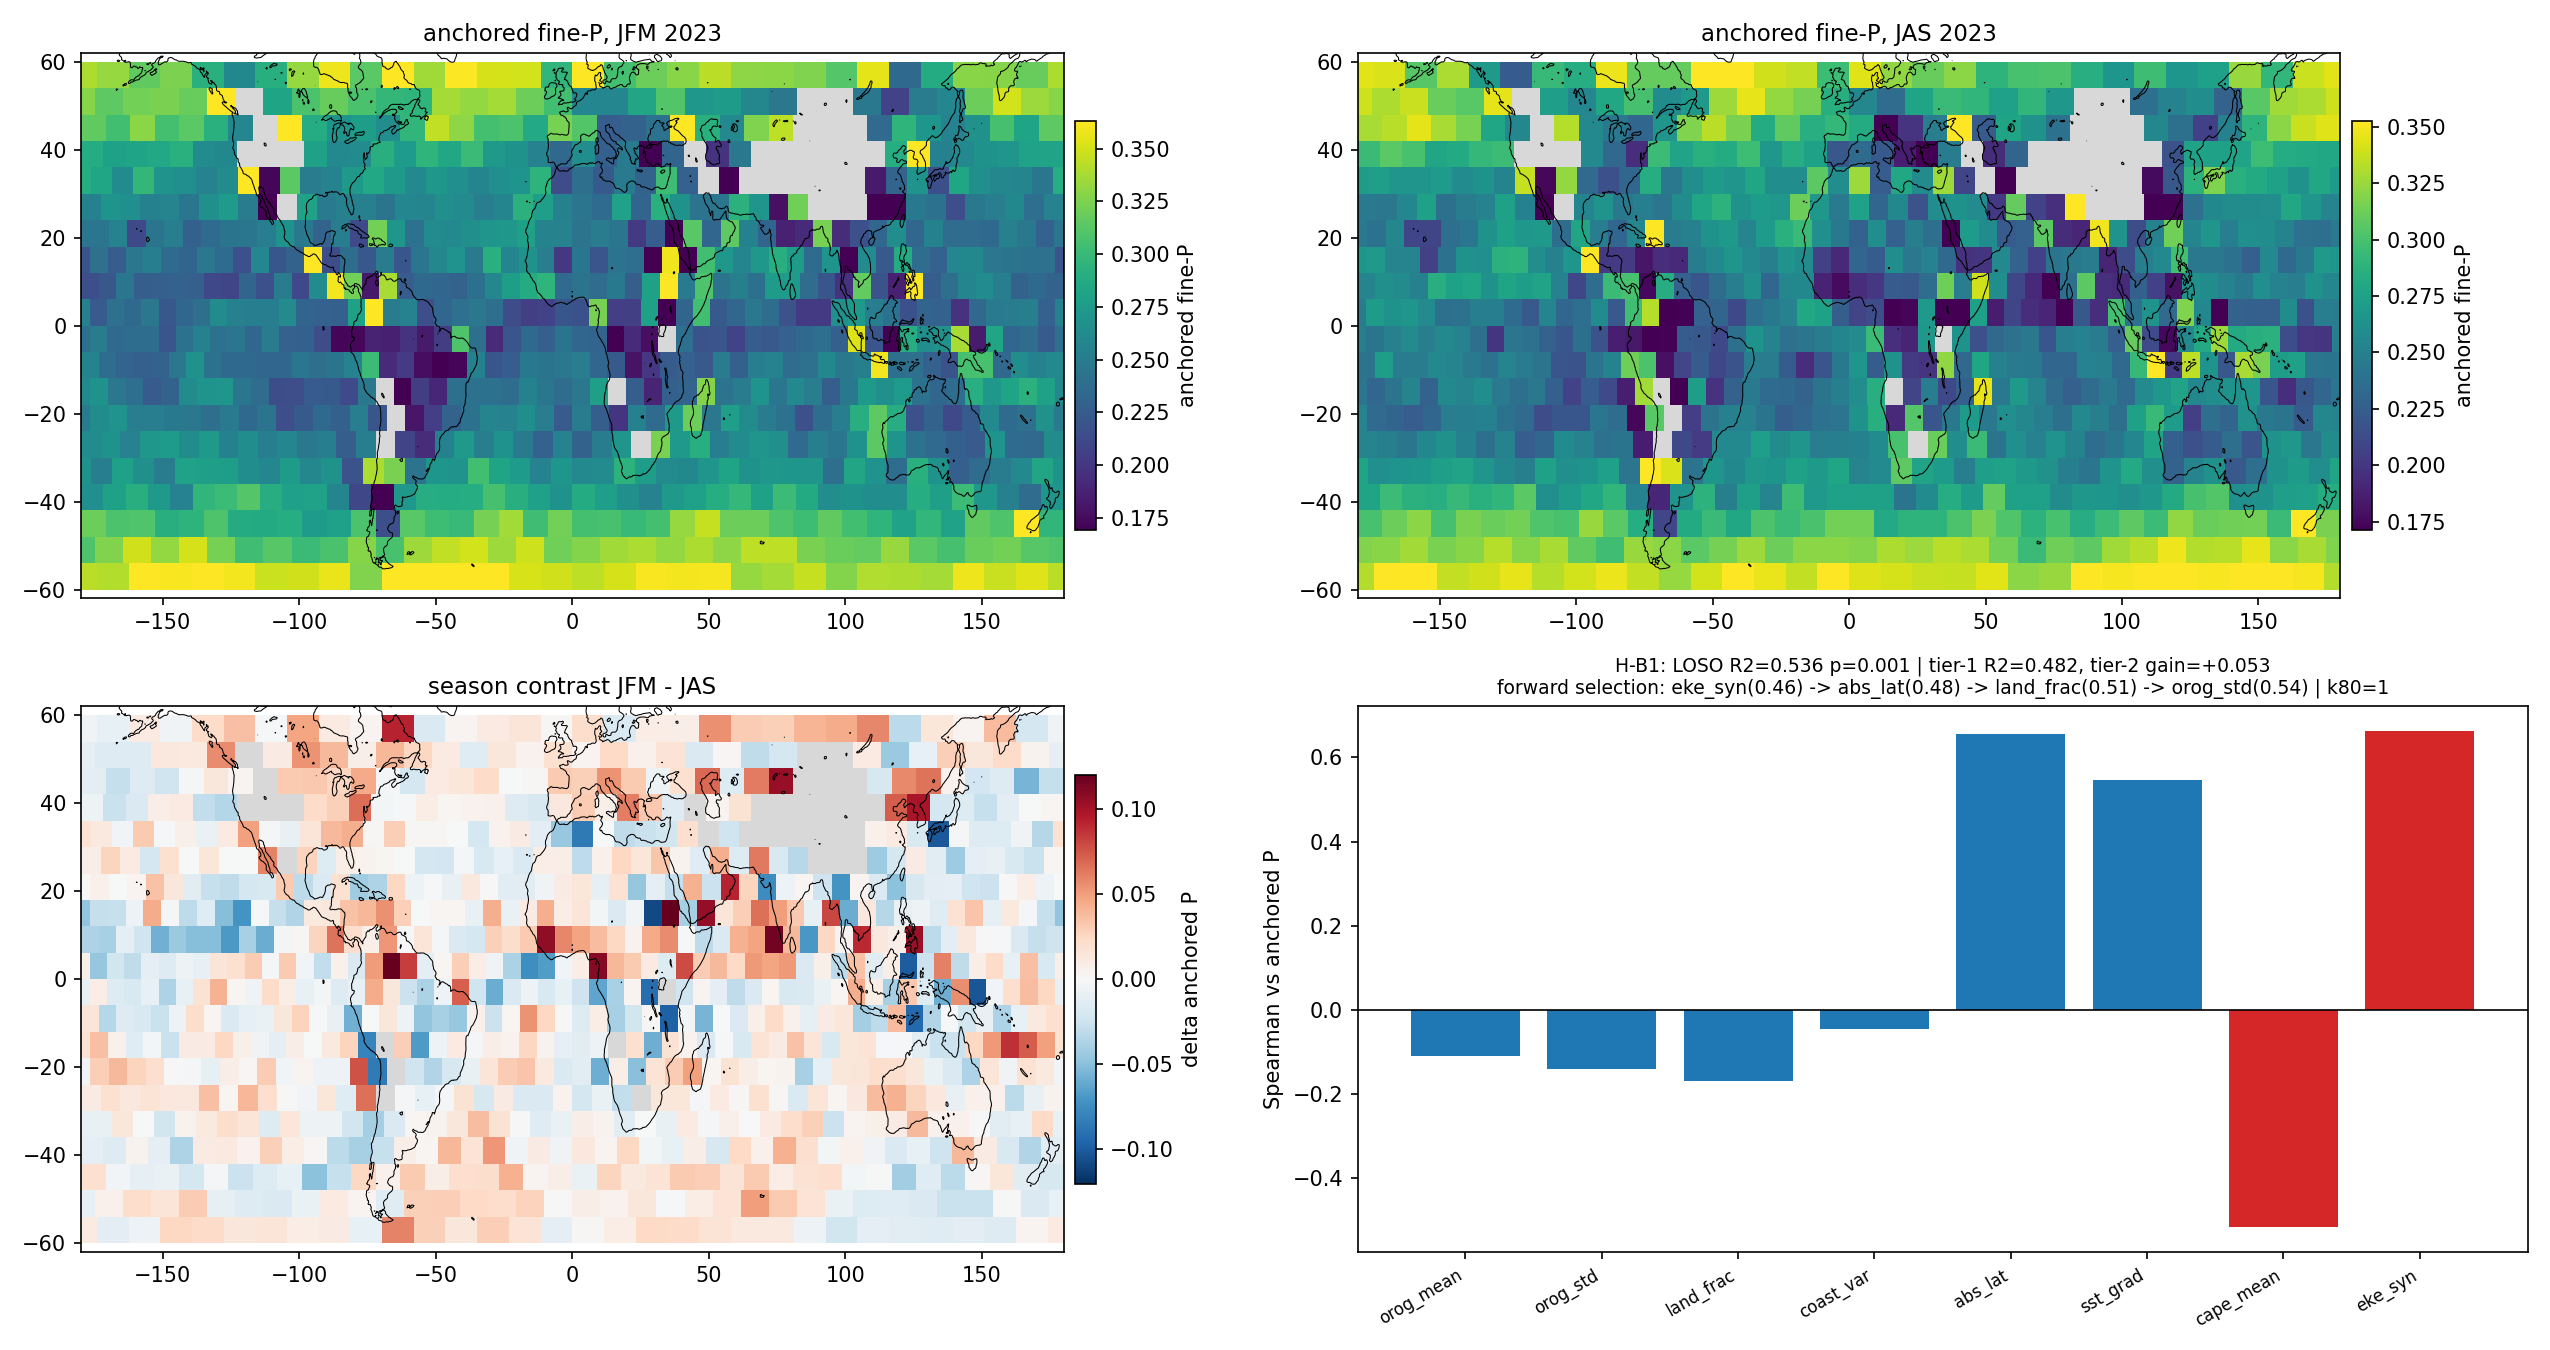
\includegraphics[width=\linewidth]{figures/fig2_seasons_attribution.png}
\caption{Часть B, сезонная структура и атрибуция: карты $P$ (с суррогатной поправкой) по сезонам январь--март и июль--сентябрь 2023~г. (вверху), сезонный контраст (внизу слева; медиана модуля 0,016) и нагрузки восьми ковариат с кривой пошагового отбора (внизу справа): вихревая энергия одна даёт $R^2=0{,}456$ из полных $0{,}536$.}
\label{fig:seasons}
\end{figure}

\subsection{Природа карты: свободный модельный расчёт}
\label{sec:model}

Сопоставление двух реанализов не отделяет свойство атмосферы от свойства наблюдательной сети: обе системы усваивают в основном одни и те же наблюдения \cite{Hersbach2020,Gelaro2017}; решающая проверка --- расчёт, не усваивающий наблюдений. Использован эксперимент \texttt{highresSST-present} проекта HighResMIP \cite{Haarsma2016} по модели ECMWF-IFS-HR \cite{Roberts2018}: расчёт типа AMIP --- атмосфера при заданной наблюдаемой температуре поверхности океана \cite{Gates1992}; глобальные поля 2014~г., разрешение $0{,}5^\circ$, без усвоения атмосферных наблюдений.

На 902 тайлах, согласованных по разрешению, ранговая корреляция эталонной пары <<ERA5 при $0{,}25^\circ$ --- ERA5 при $0{,}5^\circ$>> (одна и та же атмосфера, цена огрубления метода) составляет $0{,}897$ --- это разрешающий предел сопоставления. Карта свободного расчёта воспроизводит карту ERA5 с $\rho=0{,}869$, то есть \emph{97\,\% достижимого согласия} (здесь и далее --- отношение ранговых корреляций, а не доля объяснённой дисперсии), при том что расчёт относится к другому году (2014 против 2023) и не видел ни одного атмосферного наблюдения (рис.~\ref{fig:round2}, слева). Нагрузки ковариат на модельную карту повторяют реанализные: вихревая энергия $+0{,}68$; модуль широты $+0{,}70$; градиент ТПО $+0{,}51$; CAPE $-0{,}50$; орография $\approx0$. Глобальная карта сопряжённости --- свойство физики атмосферы при заданных граничных условиях, а не артефакт наблюдательной сети или системы усвоения.

Во избежание путаницы при совместном чтении с первой статьёй серии: там для сопоставления со свободным расчётом приводится величина $\rho=0{,}71$ при пределе $0{,}93$ --- она относится к \emph{региональной} выборке по 39 областям (2017--2024~гг.). Приведённая здесь пара $0{,}869/0{,}897$ относится к \emph{глобальной мозаичной} выборке (902 тайла, $0{,}5^\circ$, 2014 против 2023~гг.); эти величины получены на разных выборках и не взаимозаменяемы.

\begin{figure}[t]
\centering
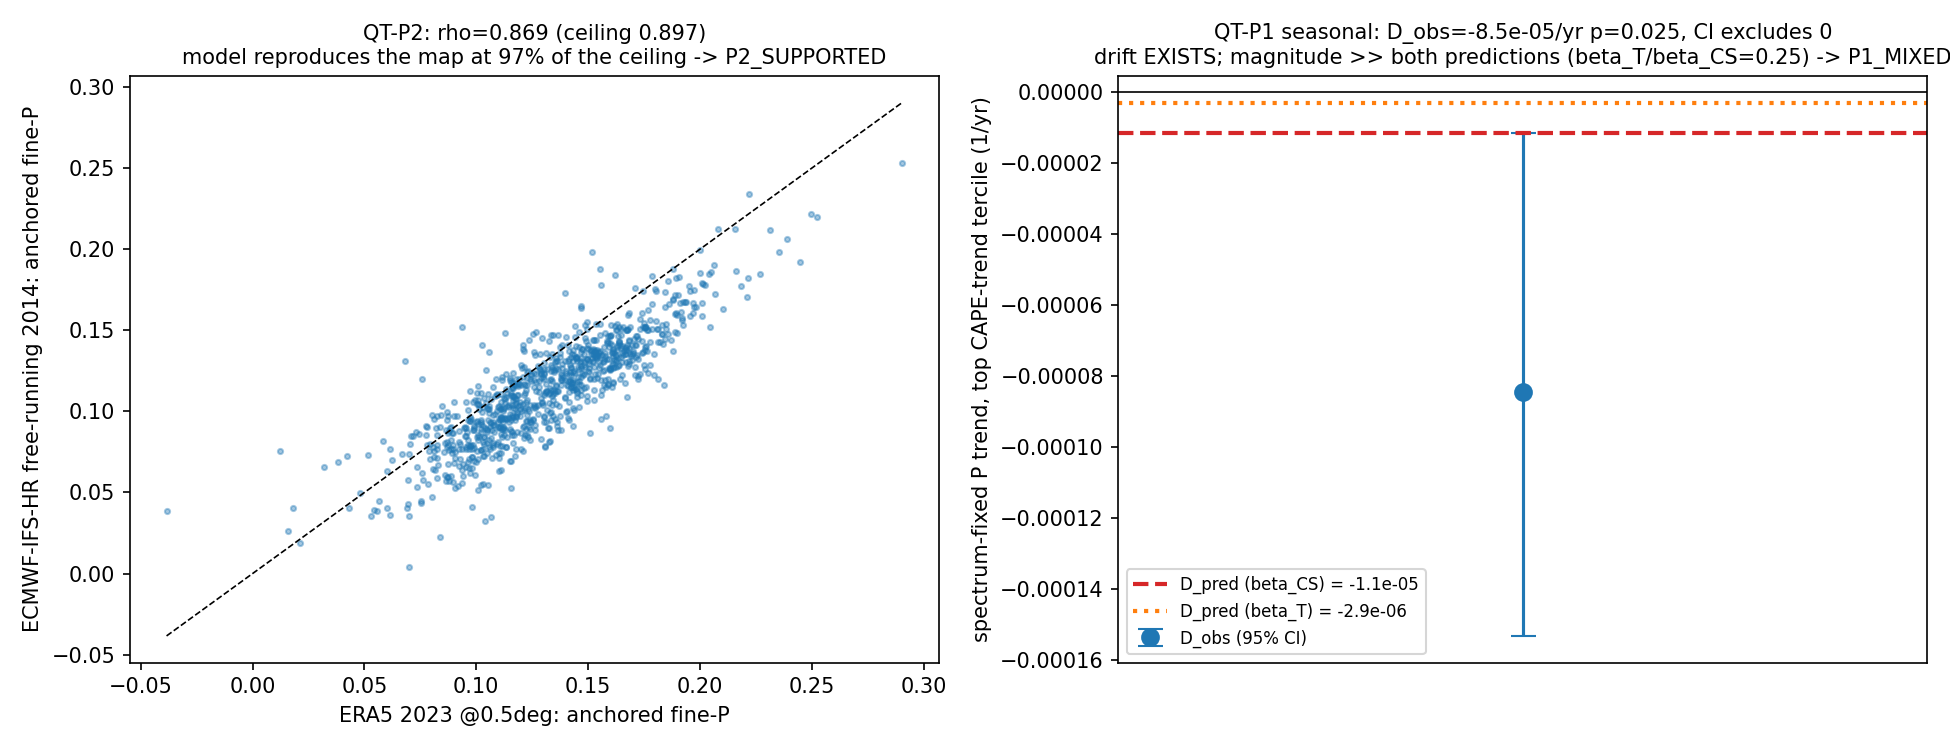
\includegraphics[width=\linewidth]{figures/fig2_qt_round2.png}
\caption{Слева: тайловая карта $P$ (с суррогатной поправкой) свободного расчёта ECMWF-IFS-HR (2014~г., без усвоения наблюдений) против карты ERA5 (2023~г.) на 902 согласованных по разрешению тайлах: $\rho=0{,}869$ при разрешающем пределе $0{,}897$; пунктир --- линия равенства. Справа: тренд спектрально-фиксированного $P$ в тайлах верхней терцили тренда CAPE (точка --- оценка, отрезок --- 95-\%-й доверительный интервал кластерного бутстрэпа) в сравнении с двумя калибровочными предсказаниями (штриховые линии); к разд.~\ref{sec:static}.}
\label{fig:round2}
\end{figure}

\subsection{Тропический избыток межгодовой изменчивости и Междекадное тихоокеанское колебание}
\label{sec:ipo}

На длинной записи (1979--2024~гг.) двенадцать областей программы демонстрируют замечательную стабильность межгодовых значений инварианта, за одним исключением: ровно три очага глубокой конвекции --- западная тропическая тихоокеанская тёплая аномалия, Амазония и юго-западная тропическая зона конвергенции Тихого океана --- несут избыток межгодовой дисперсии карт активности ($F=1{,}5$--$1{,}8$ против $F\approx1$ у остальных девяти), устойчивый к смене единицы выборки. Связь этого избытка с ЭНСО (индекс ONI \cite{Trenberth1997}) исключена прямым тестом при тридцатикратном превышении статистической мощности относительно первоначальной восьмилетней проверки (2017--2024~гг.).

Для атрибуции избытка заранее --- до обращения к данным --- был назван список из четырёх климатических индексов (PDO \cite{Newman2016}, AMO, DMI, IPO-TPI \cite{Henley2015}); статистика теста --- максимум ранговой корреляции по восьми комбинациям <<индекс $\times$ сглаживание>> с совместным нулём циклического сдвига по времени, штрафующим за множественность выбора. Результаты --- в табл.~\ref{tab:ipo} и на рис.~\ref{fig:ipo}.

\begin{table}[t]
\centering
\caption{Атрибуция тропического избытка межгодовой изменчивости по заранее названным индексам (максимум-статистика по 8 комбинациям <<индекс $\times$ сглаживание>>, совместный нуль циклического сдвига).}
\label{tab:ipo}
\small
\begin{tabular}{@{}lcccc@{}}
\toprule
Регион & $T=\max\lvert\rho\rvert$ & Лучший индекс & $p$ & Значимо\\
\midrule
Зап. тропическая Пацифика (тёплая аномалия) & 0,311 & PDO (5-летнее сглаж.) & 0,155 & нет\\
Амазония & 0,453 & IPO-TPI & 0,001 & да\\
Юго-зап. зона конвергенции Тихого океана & 0,602 & IPO-TPI & 0,001 & да\\
\bottomrule
\end{tabular}
\end{table}

Совпадение ведущего индекса в двух из трёх регионов активирует заранее зафиксированное правило согласованности: тропический избыток --- проявление \emph{декадной} моды, Междекадного тихоокеанского колебания (IPO) \cite{Power1999,Henley2015}, а не межгодового ЭНСО-режима. Третий регион (тёплая аномалия запада Пацифики, самый слабый избыток) остаётся неатрибутированным.

\begin{figure}[t]
\centering
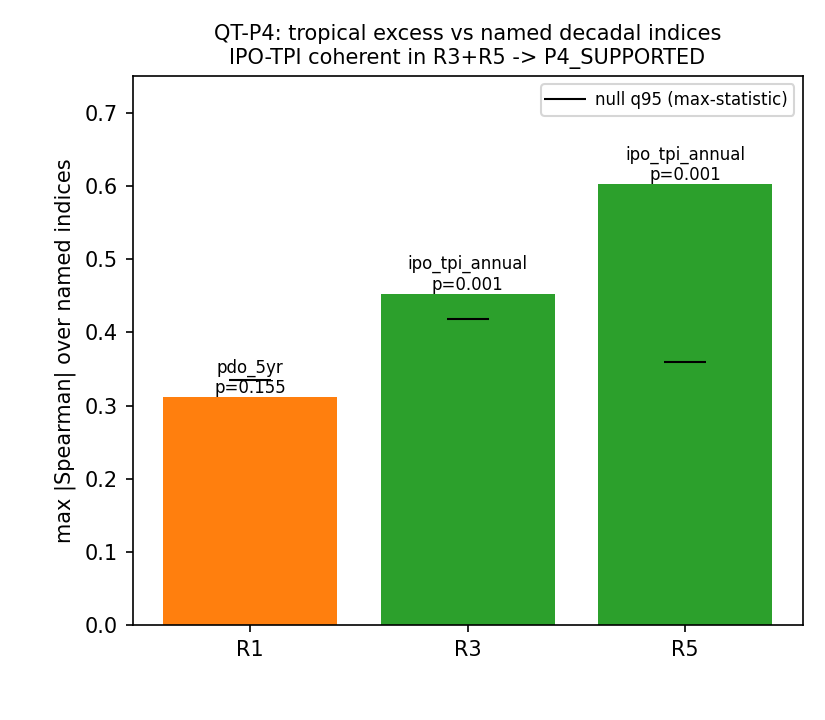
\includegraphics[width=0.6\linewidth]{figures/fig2_ipo.png}
\caption{Максимум-статистика связи межгодовой дисперсии карт активности с заранее названными климатическими индексами для трёх очагов тропического избытка; горизонтальные отрезки --- 95-е перцентили совместного нуля циклического сдвига. В Амазонии (R3) и юго-западной зоне конвергенции (R5) значим один и тот же индекс --- IPO-TPI.}
\label{fig:ipo}
\end{figure}

\section{Интерпретация: макропеременная совместно сложившихся условий}
\label{sec:interp}

Разделение ковариат на ярусы задаёт и допустимый язык итоговой интерпретации. Для яруса~1 --- орографии, конфигурации суши и океана, широты, градиента температуры поверхности океана --- направленная формулировка <<граничные условия формируют географию сопряжённости>> корректна: эти поля экзогенны по отношению к циркуляции на любых рассматриваемых временных масштабах. Для яруса~2 --- синоптической вихревой активности и конвективного режима --- направленный язык не используется: их связь с~$P$ пикирует на нулевом сдвиге без опережения в какую-либо сторону, и корректная формулировка --- \emph{совместное формирование}: сопряжённость уровней, штормовая активность и конвективный режим суть согласованные проявления одной установившейся организации циркуляции, а не звенья причинной цепи друг для друга. С этим согласуется и то, что один ярус~1 даёт $R^2=0{,}482$ из итоговых $0{,}536$: граничные условия и совместно сложившееся состояние читают, по существу, одну и ту же карту с разных сторон. Профиль при этом естественно читать как наблюдаемую проекцию установившейся статистики быстрой динамики циркуляции при фиксированном на масштабе наблюдения поле внешних условий; развёртывание этой интерпретации, её следствия и границы применимости --- предмет третьей статьи серии и за пределы настоящего абзаца здесь не выходят.

\section{Проверка гипотезы статичности}
\label{sec:static}

Если~$P$ --- статичная характеристика сложившегося режима, он по определению не должен опережать перестройку этого режима и не должен превосходить по чувствительности стандартные показатели среднего поля. Это следствие проверено прямо; итоги сведены в табл.~\ref{tab:static}.

\emph{Реакция на известную перестройку режима.} Единственный крупный документированный сдвиг внутри записи --- переход Междекадного тихоокеанского колебания 1998/99~гг. На 72 парах <<тайл--сезон>> трёх тропических регионов сопоставлены статистики перехода четырёх показателей. Доля случаев, в которых~$P$ реагирует на переход раньше или резче конкурента, составила: против CAPE --- 25\,\%, против синоптической вихревой энергии --- 47\,\%, против наклона спектра --- 42\,\% при пороге опережающего поведения 60\,\%. По медианному отношению <<сигнал/шум>> многолетнего тренда на 288 парах <<тайл--сезон>> $P$ занимает последнее место из четырёх: CAPE --- 2,39; наклон спектра --- 1,03; вихревая энергия --- 0,85; $P$ --- 0,67 (все парные сравнения значимы). Для инварианта, по построению не несущего собственной динамики, это ожидаемое поведение, прямо подтверждающее исходную гипотезу: величина регистрирует архитектуру уже сложившегося режима и не выступает опережающим индикатором его перестройки.

\emph{Отдельный и открытый вопрос --- многодесятилетняя устойчивость самого инварианта.} На сезонной выборке (288 пар <<тайл--сезон>>, не менее 30 лет каждая) в тайлах верхней терцили тренда CAPE обнаружен слабый отрицательный тренд спектрально-фиксированного~$P$: $-8{,}5\cdot10^{-5}$~год$^{-1}$, $p=0{,}025$, доверительный интервал кластерного бутстрэпа исключает ноль (рис.~\ref{fig:round2}, справа). Величина тренда примерно в семь раз превышает кросс-секционную калибровку по пространственному контрасту CAPE и на порядок --- калибровку по межгодовой ковариации: отклик, если он реален, зависит от временного масштаба воздействия. Однако единственный доступный свободный расчёт с переходным форсингом воспроизводит тренд того же знака лишь на $\sim$27\,\% величины и статистически неотличим от нуля ($p=0{,}221$). Это вопрос иного типа, чем предсказательная сила: речь о стабильности самих условий, задающих инвариант, на масштабе десятилетий. На сегодняшних данных он не решён: факт тренда установлен только внутри ERA5 --- записи, охватывающей крупные смены наблюдательной системы, --- и модельное подтверждение его физической природы отсутствует. Мы оставляем статус вопроса явно открытым.

\begin{table}[t]
\centering
\caption{Сводка проверки гипотезы статичности инварианта.}
\label{tab:static}
\small
\begin{tabular}{@{}p{0.47\linewidth}p{0.47\linewidth}@{}}
\toprule
Проверка & Итог\\
\midrule
Опережает ли $P$ стандартные показатели на переходе 1998/99~гг. (порог 60\,\%) & нет: опережение против CAPE в 25\,\% случаев, против вихревой энергии в 47\,\%, против наклона спектра в 42\,\% --- согласуется с гипотезой статичности\\
Чувствительность к многолетнему тренду (медианное сигнал/шум, 288 пар <<тайл--сезон>>) & $P$ --- последний из четырёх показателей: 0,67 против 2,39 (CAPE), 1,03 (наклон), 0,85 (вихревая энергия)\\
Тренд спектрально-фиксированного $P$ в тайлах наибольшего тренда CAPE (ERA5) & $-8{,}5\cdot10^{-5}$~год$^{-1}$, $p=0{,}025$, доверительный интервал исключает ноль\\
Тот же тренд в свободном расчёте с переходным форсингом & тот же знак при $\sim$27\,\% величины, $p=0{,}221$ --- физичность тренда не подтверждена, вопрос открыт\\
\bottomrule
\end{tabular}
\end{table}

\section{Обсуждение и ограничения}
\label{sec:limitations}

Совокупность результатов складывается в определённый статус величины: география сопряжённости уровней --- не случайный рисунок и не артефакт наблюдательной системы, а физически атрибутируемая, эффективно одномерная и воспроизводимая карта, читаемая на языке известных организаторов циркуляции. Пять ограничений заслуживают явной фиксации.

Во-первых, тонкие полосы 50--400~км частично или полностью лежат ниже эффективного разрешения реанализа (разд.~\ref{sec:data}); аргументы разд.~\ref{sec:data} показывают, что карта не является артефактом одного вычислительного тракта, но величина остаётся определённой операционально --- на выходе систем класса реанализа и глобальной модели ($0{,}25$--$0{,}5^\circ$); её перенос на наблюдения километрового разрешения --- открытый вопрос.

Во-вторых, глобальная карта построена по одному году (2023) и двум сезонам. Смягчающие обстоятельства --- сезонная устойчивость карты (медиана контраста 0,016), согласованность с частью~A, охватывающей окна 2021--2024~гг., и воспроизведение карты модельным расчётом 2014~г.; многолетняя глобальная карта остаётся задачей отдельной работы.

В-третьих, проверка природы карты опирается на один свободный расчёт одной модели; желательное усиление --- ансамбль реализаций и модель с иным динамическим ядром.

В-четвёртых, синоптическая вихревая энергия вычисляется из того же поля ветра, что и сам профиль, --- это два разных функционала одних данных. Верхнюю границу возможной инфляции связи даёт атрибуция только по независимым полям яруса~1: $R^2=0{,}482$ из полных $0{,}536$.

В-пятых, многолетний тренд спектрально-фиксированного профиля установлен только внутри ERA5 --- записи, охватывающей крупные смены наблюдательной системы, --- и не подтверждён свободным расчётом (разд.~\ref{sec:static}); его статус остаётся открытым.

\section{Выводы}
\label{sec:conclusion}

1.~Переход от 39 региональных областей к мозаичной карте (144, затем 936 тайлов) решает проблему малой выборки, погубившую первую попытку атрибуции, и впервые делает атрибуцию географии сопряжённости уровней статистически честной: предсказание проверяется на целиком выбывающих регионах и секторах долготы, нуль-модель сохраняет пространственную автокорреляцию, критерии зафиксированы до вычислений.

2.~География инварианта атрибутируется внешним ковариатам на двух независимых выборках с согласованными знаками и величинами ($R^2=0{,}40$ и $0{,}54$, $p=0{,}001$). Механизм двухканален: синоптическая штормовая активность повышает сопряжённость через ту же дисперсионную структуру, которую отражает спектр; конвективный режим понижает её сверх спектра. Атрибуция сопряжённости не сводится к атрибуции спектра: у двух мишеней разные ведущие ковариаты.

3.~Глобальная карта эффективно одномерна (одна ковариата --- синоптическая вихревая энергия --- даёт 85\,\% качества предсказания) и воспроизводится свободным модельным расчётом без усвоения наблюдений на 97\,\% достижимого согласия ($\rho=0{,}869$ при разрешающем пределе $0{,}897$): карта отражает физику атмосферы, а не устройство наблюдательной сети.

4.~Потолок надёжности карты составляет $R^2=0{,}914$ (внутрисезонное расщепление выборки пополам); восемь заявленных ковариат объясняют 59\,\% воспроизводимой дисперсии, добавление статистик интермиттентности --- 83\,\%; остаток воспроизводим, не спектрален и географически организован --- его источники заявлены задачей дальнейшей работы. Биологический отрицательный контроль чист.

5.~Тропический избыток межгодовой изменчивости в двух из трёх очагов глубокой конвекции статистически связан с Междекадным тихоокеанским колебанием (IPO-TPI, $p=0{,}001$ в обоих регионах при совместном нуле с поправкой на множественность); связь с ЭНСО исключена при тридцатикратном превышении мощности.

6.~Гипотеза статичности инварианта подтверждена прямой проверкой: на известной перестройке циркуляции 1998/99~гг. величина не опережает и не превосходит по чувствительности стандартные показатели режима --- ожидаемое поведение характеристики, не несущей собственной динамики. Вопрос о медленном многодесятилетнем дрейфе самих условий, задающих инвариант, остаётся открытым: тренд обнаружен только внутри ERA5 и не подтверждён свободным расчётом. Итоговый статус величины, складывающийся из первой статьи серии и настоящей работы: воспроизводимая, физически атрибутируемая, глобально картируемая макропеременная сложившихся условий циркуляции; её более широкая теоретическая интерпретация --- предмет завершающей статьи серии.

\paragraph{Доступность данных и кода.} Исходные данные --- открыто доступные продукты сторонних поставщиков и в репозитории автора не дублируются: поля ERA5 доступны через Climate Data Store (Copernicus Climate Change Service), модельные расчёты HighResMIP --- через Earth System Grid Federation, ряды климатических индексов --- через NOAA PSL; доступ к CDS требует бесплатной учётной записи. Код анализа, скрипты получения данных, зафиксированные до вычислений протоколы обеих частей, журнал отступлений и производные табличные результаты, достаточные для воспроизведения всех рисунков и статистических проверок работы, открыты в репозитории \url{https://github.com/Theclimateguy/Shroedinger} (версия v6.2; постоянный архив версий --- Zenodo, DOI 10.5281/zenodo.19565769). Маршрут воспроизведения статьи --- от получения данных до каждой таблицы и рисунка --- описан в файле \texttt{reproducibility/article2\_README.md} и автоматизирован скриптом \texttt{reproducibility/reproduce\_article2.py}; там же приведены контрольные суммы ожидаемых артефактов.

\printbibliography[title={Список литературы}]

\end{document}
